% !TEX root = recommending-interesting-writing.tex
\section{Introduction}
\label{sec:introduction}
Creative nonfiction, longform journalism, and blog posts are examples of the types of articles curated by The Browser's team of editors. The editors read a large number of articles from various publications to select content to recommend to subscribers.

In building a recommender system to help editors sift through many documents, it is motivating to highlight the trade-off in user privacy intrinsic to recommender systems. A machine learning model must exploit information about a user. However, the incentive structures of operating a recommender system within a business can influence decisions around privacy and transparency~\citep{diakopoulos2020oxford}. For example, business models that rely on online advertising may engender recommender systems that upweight attention-grabbing content and hence time spent looking at ads. Such content might maximize a user's time spent with a service over time at the expense of long-term user experience or consent. In comparison, privacy-preserving and open source tools such as the Signal encrypted messaging service\footnote{\url{https://signal.org/}} may provide improved user experience in terms of privacy-preserving, transparent, and explainable algorithms and visual interfaces~\citep{cohn-gordon2017a-formal}. But the incentive structures for releasing recommender systems and visual interfaces that exploit private information about users are poor. There are few examples of end-to-end, open source, free-to-deploy pipelines for recommending content to users using a visual interface. This motivates building and deploying a recommendation model and corresponding explanation-aware visual interface to give users control, and inform them about how data is being used to make recommendations.

We build an end-to-end recommender system visual interface to address two aims: (1) to aid editors at The Browser in their decision-making task, and give them control through an explanation-aware interface, and (2) to release a lightweight, performant, open-source visual interface framework for explanation-aware recommender systems for document recommendation. In an offline evaluation, we show that the recommendation model we use for the visual interface outperforms \acrshort{bert}, a competitive document classification model. In a qualitative study, the control and explanations provided by the visual interface help editors in their decision-making and help find bugs in the recommendation model.

% !TEX root = ../recommending-interesting-writing.tex
\begin{figure}[!tb]
  \centering
  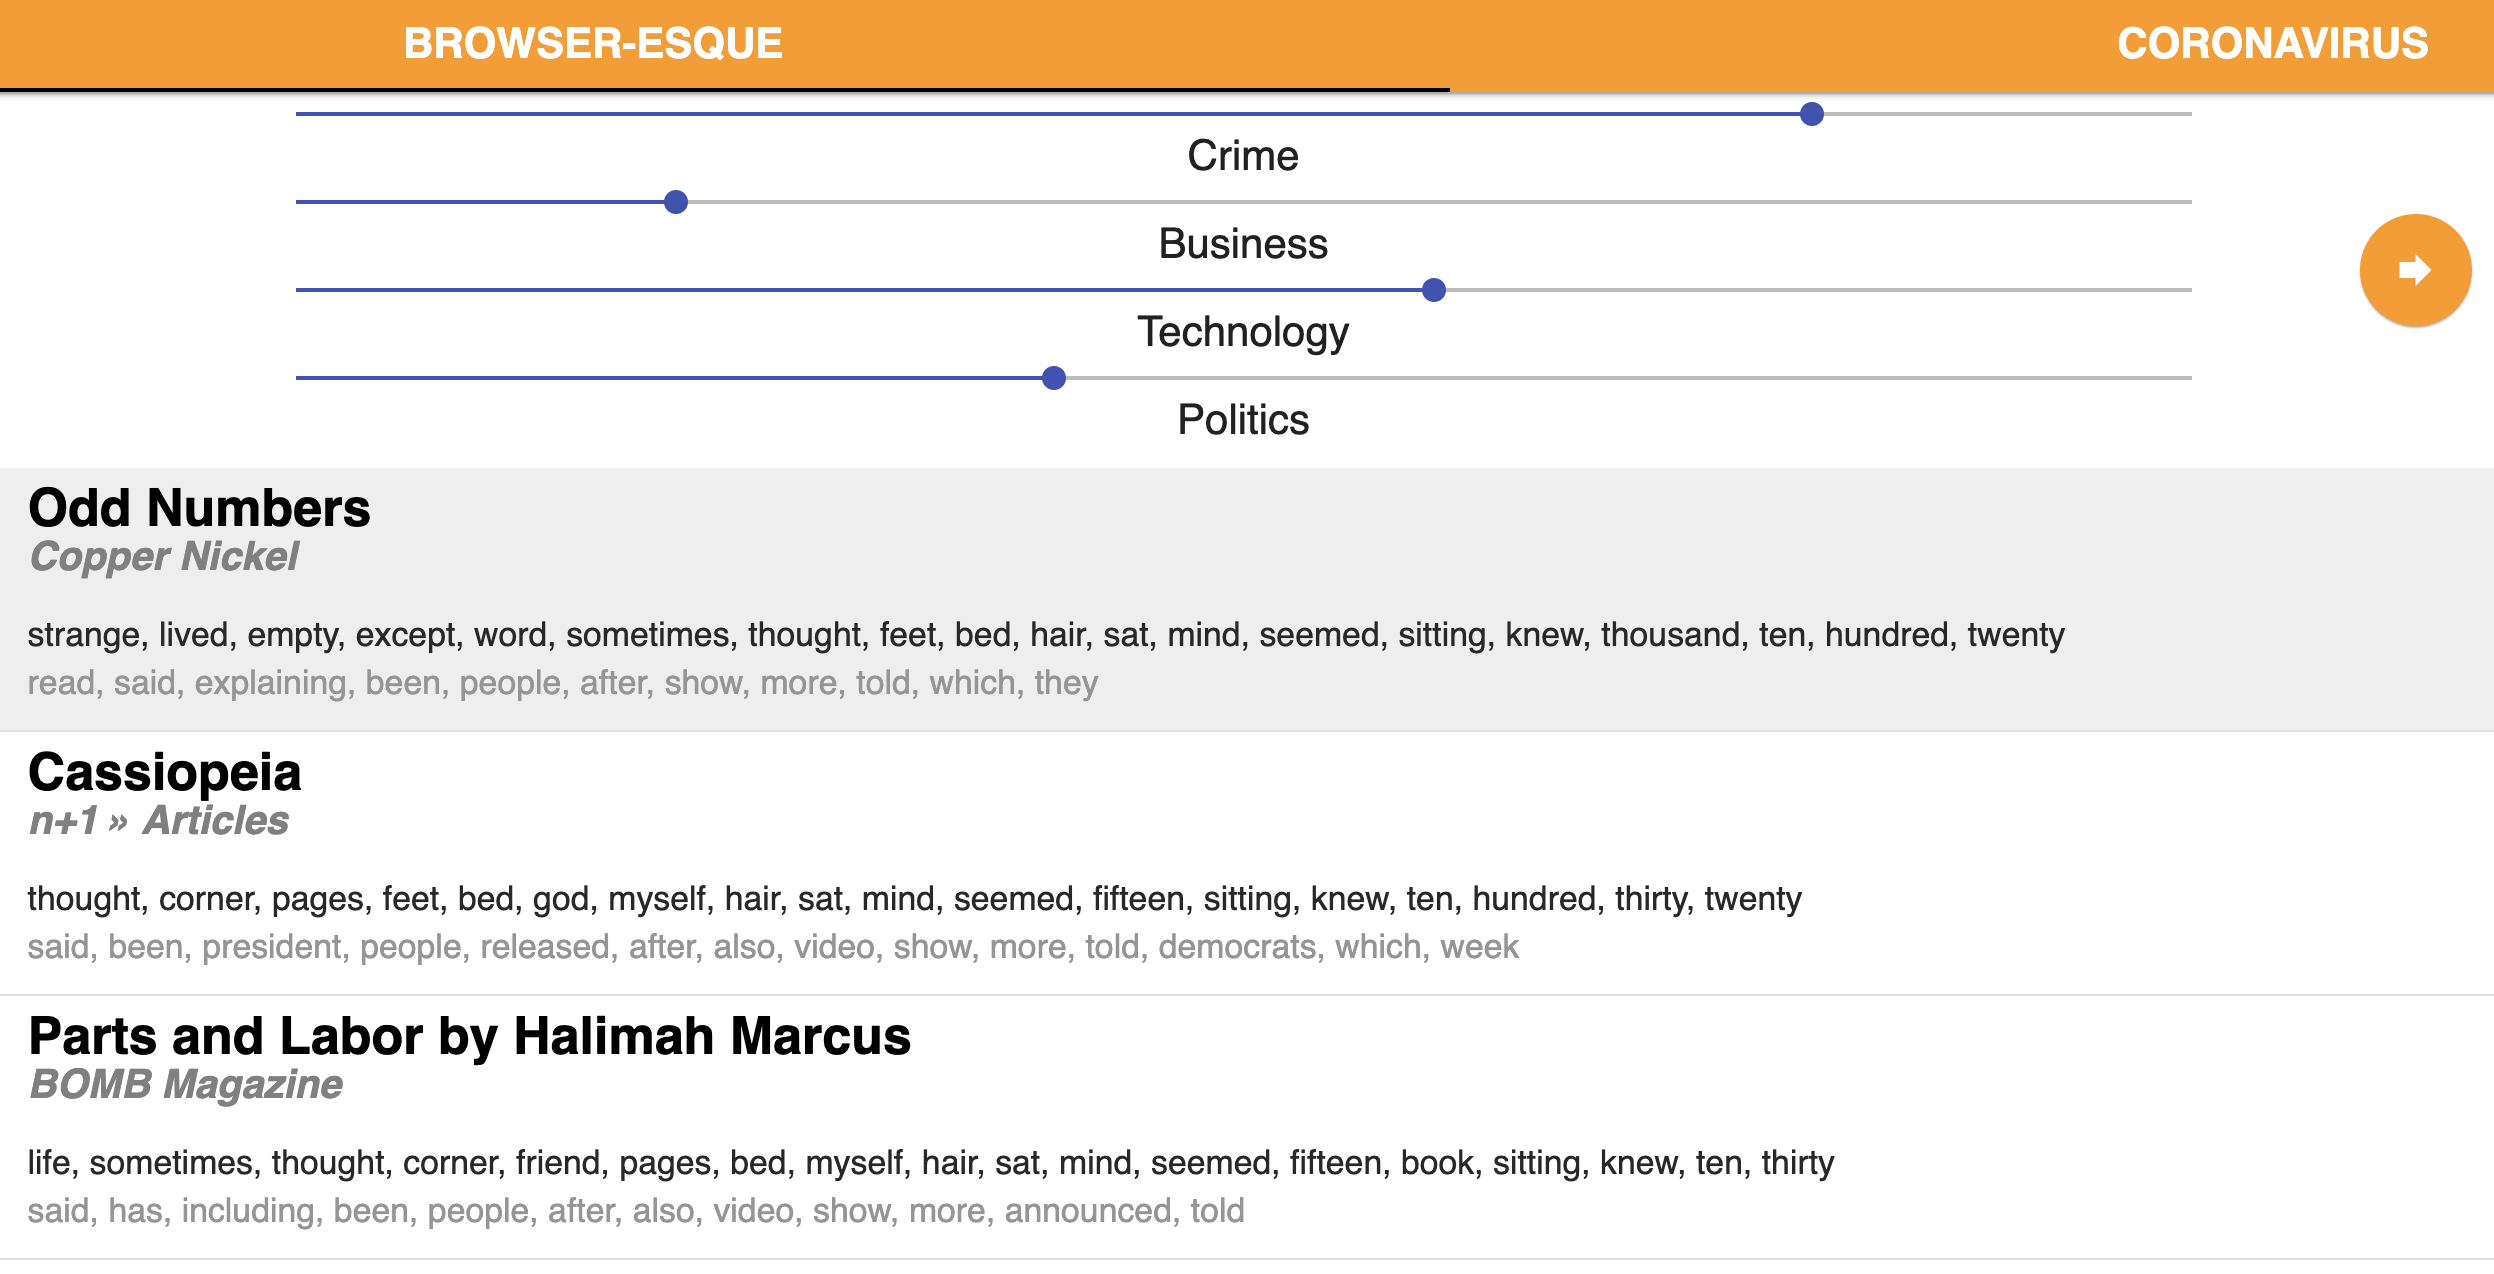
\includegraphics[width=\linewidth]{fig/screen_shots/screen_shot_10.png}
  \caption{Visual interface to \acrlong{rfs} includes topic sliders for setting user preferences as well as most important topic words for each found article}
  \label{fig:screen-shot}
\end{figure}